
\de{ĐỀ THI HỌC KỲ I NĂM HỌC 2022-2023}{THPT Giồng Ông Tố}
\begin{center}
	\textbf{PHẦN 1 - TRẮC NGHIỆM}
\end{center}
\Opensolutionfile{ans}[ans/ans]
\begin{ex}%[0T6Y2-1]%[Dự án đề kiểm tra HKI NH22-23- Hieu Phan]%[THPT GIỒNG ÔNG TỐ]
    Để điều tra các con trong mỗi gia đình của một chung cư gồm $ 100 $ gia đình. Người ta chọn ra $ 20 $ gia đình ở tầng 4 và thu được mẫu số liệu sau đây: $ 2\,\, 4\,\, 2 \,\,1 \,\,3\,\, 5 \,\,1 \,\,1 \,\,2 \,\,3 \,\,1\,\, 2\,\, 2 \,\,3 \,\,4 \,\,1\,\, 1 \,\,2 \,\,3\,\, 4 $. Có bao nhiêu giá trị khác nhau trong mẫu số liệu trên?
    \choice
    {$ 4 $}
    {$ 10 $}
    {\True $ 5 $}
    {$ 20 $}  
    \loigiai
    {
        Từ mẫu số liệu ta thấy có $ 5 $ giá trị khác nhau là $ 1\,\,2\,\,3\,\,4\,\,5 $.
    }
\end{ex}
\begin{ex}%[0T4B2-1]%[Dự án đề kiểm tra HKI NH22-23- Hieu Phan]%[THPT GIỒNG ÔNG TỐ]
    Tam giác $ ABC $ có $ AB=2, AC=1 $ và $ \widehat{A}=60^\circ $. Tính độ dài cạnh $ BC $.
    \choice
    {$ BC=1 $}
    {$ BC=2 $}
    {\True $ BC=\sqrt{3} $}
    {$ BC=\sqrt{2} $}  
    \loigiai
    {
        Ta có $ BC=\sqrt{AB^2+AC^2-2\cdot AB\cdot AC\cdot \cos \widehat{A} }=\sqrt{2^2+1^2-2\cdot 2\cdot 1\cdot \cos 60^\circ } =\sqrt{3}$.
    }
\end{ex}
\begin{ex}%[0T5B1-2]%[Dự án đề kiểm tra HKI NH22-23- Hieu Phan]%[THPT GIỒNG ÔNG TỐ]
Cho hai  véc-tơ $ \vec{a} $ và $ \vec{b} $ không cùng phương. Hai véc-tơ nào sau đây cùng phương?
\choice
{$ -\dfrac{1}{2}\vec{a}-\vec{b} $ và $ 2\vec{a}+\vec{b} $}
{\True $ \dfrac{1}{2}\vec{a}-\vec{b} $ và $ -\dfrac{1}{2}\vec{a}+\vec{b} $}
{$-3\vec{a}+\vec{b} $ và $ -\dfrac{1}{2}\vec{a}+6\vec{b} $}
{$ \dfrac{1}{2}\vec{a}+\vec{b} $ và $ \vec{a}-2\vec{b} $}  
\loigiai
{
    Ta có $ \dfrac{1}{2}\vec{a}-\vec{b}=-\left(-\dfrac{1}{2}\vec{a}+\vec{b}\right) $ nên suy ra hai véc-tơ này cùng phương.
}
\end{ex}
\begin{ex}%[0T2Y1-1]%[Dự án đề kiểm tra HKI NH22-23- Hieu Phan]%[THPT GIỒNG ÔNG TỐ]
    Bạn Nam để dành được $ 800 $ nghìn đồng. Trong đợt quyên góp ủng hộ miền Trung sau đợt lũ lụt, bạn Nam đã đóng góp $ x $ tờ $ 20 $ nghìn và $ y $ tờ $ 50 $ nghìn. Bất phương trình thể hiện mối liên hệ của $ x $ và $ y $ là
    \choice
    {$ 50x+20y\le 800 $}
    {$ 50x+20y\ge 800 $}
    {$ 20x+50y\ge 800 $}
    {\True $ 20x+50y\le 800 $}  
    \loigiai
    {
        Số tiền bạn Nam ủng hộ là $ 20x+50y $.\\
        Theo đề bài ta có $ 20x+50y \le 800 $.
    }
\end{ex}
\begin{ex}%[0T2B2-3]%[Dự án đề kiểm tra HKI NH22-23- Hieu Phan]%[THPT GIỒNG ÔNG TỐ]
    Phần không tô đậm trong hình vẽ dưới đây (không chứa biên) biểu diễn tập nghiệm của hệ bất phương trình nào trong các hệ bất phương trình sau?
    \begin{center}
       % Đồ thị hàm y=ax+b. Nếu hệ số lớn cần điều chỉnh hệ trục, vùng lưới, domain và lệnh \clip
       \begin{tikzpicture}[>=stealth,x=1cm,y=1cm,scale=1]
           \draw[->] (-3,0) -- (2.8,0) node[below] {\scriptsize $x$};
           \draw[->] (0,-2.5) -- (0,2.5) node[left] {\scriptsize $y$};
           \draw (0,0)node[below right]{\scriptsize $O$};
           \clip (-3,-3)rectangle(3,3);
          
           \draw[thick,samples=150,smooth,domain=-3:2.5] plot(\x,{(-0.333)*\x+(-0.666)});
           \fill[pattern=north east lines,smooth] (-3,-2) --plot[domain=-3:2.5] (\x,{(-0.333)*\x+(-0.666)})
           -- (2.5,-2) -- cycle;
            \draw[thick, samples=150,smooth,domain=-3:2.5] plot(\x,{(0.5)*\x});
            \fill[pattern=north east lines,smooth] (-3,-2) --plot[domain=-3:2.5] (\x,{(0.5)*\x})-- (2.5,-2) -- cycle;
            \draw[dashed,thin] (2,0)--(2,1)--(0,1);
           \foreach \x in {-2,2}\fill (\x,0)node[above right]{\scriptsize $ \x $} circle (1.2pt) ;
           \foreach \x in {1}\fill (0,\x,0)node[left]{\scriptsize $ \x $} circle (1.2pt) ;
       \end{tikzpicture}
    \end{center}
    \choice
    {$ \heva{& x-2y\le 0 \\ &x+3y\le-2 } $}
    {\True $ \heva{& x-2y< 0 \\ &x+3y>-2 } $}
    {$ \heva{& x-2y > 0 \\ &x+3y<-2 } $}
    {$ \heva{& x-2y\le 0 \\ &x+3y\ge-2 } $}  
    \loigiai
    {
        Dựa vào đồ thị ta thấy điểm $ (0,1) $ thuộc miền nghiệm của hệ bất phương trình.\\
        Vì miền nghiệm không chứa biên nên thế $ (0,1) $ vào hệ bất phương trình $$ \heva{& x-2y< 0 \\ &x+3y>-2 }\Leftrightarrow \heva{& -1 < 0 \\ & \quad3>- 2 }\text{ (thỏa).} $$ 
        Vậy bất phương trình cần tìm là $ \heva{& x-2y< 0 \\ &x+3y>-2. } $
    }
\end{ex}
\begin{ex}%[0T3B2-2]%[Dự án đề kiểm tra HKI NH22-23- Hieu Phan]%[THPT GIỒNG ÔNG TỐ]
    Cho hàm số $ y=ax^2+bx+c $ có đồ thị như hình bên. Khẳng định nào sau đây đúng?
    % Đồ thị hàm y=ax^2+bx+c. Nếu hệ số lớn cần điều chỉnh hệ trục, vùng lưới, domain và lệnh \clip
  \begin{center}
        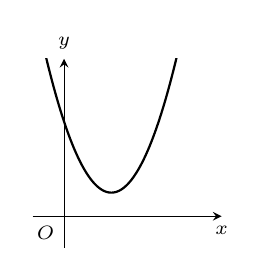
\begin{tikzpicture}[>=stealth,x=1cm,y=1cm,scale=0.4]
        \def\a{1} % Hệ số a phải khác 0
        \def\b{-3}
        \def\c{3}
        \draw[->] (-1,0) -- (5,0) node[below] {\scriptsize $x$};
        \draw[->] (0,-1) -- (0,5) node[above] {\scriptsize $y$};
        \draw (0,0)node[below left]{\scriptsize $O$};
        \pgfmathsetmacro\xdinh{-(\b)/2*(\a)}
        \pgfmathsetmacro\ydinh{(4*(\a)*(\c)-(\b)^2)/(4*(\a))}
%        \fill[dashed] (\xdinh,\ydinh)circle(2pt) edge (\xdinh,0) edge (0,\ydinh);
        \clip (-1,-1)rectangle(5,5);
        \draw[thick,samples=150,smooth,domain=-1:5] plot(\x,{\a*(\x)^2+(\b)*\x+(\c)});
    \end{tikzpicture}
    
  \end{center}
    \choice
    {\True $ a>0,b<0,c>0 $}
    {$ a<0,b<0,c>0 $}
    {$ a>0,b>0,c>0 $}
    {$ a>0,b<0,c<0 $}  
    \loigiai
    {
      Dựa vào đồ thị ta suy ra $ \heva{& (P) \text{ cắt trục Oy tại điểm }(0,c) \text{ với }c>0 \\ & \text{ bề lõm quay lên nên } a>0\\&- \dfrac{b}{2a}>0 \Rightarrow b<0.} $  \\
      Vậy $ a>0,b<0,c>0 $.
    }
\end{ex}
\begin{ex}%[0T4B1-3]%[Dự án đề kiểm tra HKI NH22-23- Hieu Phan]%[THPT GIỒNG ÔNG TỐ]
    Giá trị của biểu thức $ A=\dfrac{\cos 750^\circ+\sin 420^\circ}{\sin(-330^\circ)-\cos(-390^\circ)} $ bằng
    \choice
    {$ \dfrac{1-\sqrt{3}}{\sqrt{3}} $}
    {\True $ -3-\sqrt{3} $}
    {$ \dfrac{2\sqrt{3}}{\sqrt{3}-1} $}
    {$ 2-3\sqrt{3} $}  
    \loigiai
    {
        Ta có $ A=\dfrac{\cos 750^\circ+\sin 420^\circ}{\sin(-330^\circ)-\cos(-390^\circ)}=\dfrac{\cos 30^\circ+\sin 60^\circ}{\sin(30^\circ)-\cos(30^\circ)}=-3-\sqrt{3}$.
    }
\end{ex}
\begin{ex}%[0T3B2-2]%[Dự án đề kiểm tra HKI NH22-23- Hieu Phan]%[THPT GIỒNG ÔNG TỐ]
    Đồ thị trong hình vẽ là đồ thị của hàm số nào?
    \begin{center}
        % Đồ thị hàm y=ax^2+bx+c. Nếu hệ số lớn cần điều chỉnh hệ trục, vùng lưới, domain và lệnh \clip
        \begin{tikzpicture}[>=stealth,x=1cm,y=1cm,scale=1]
            \def\a{2} % Hệ số a phải khác 0
            \def\b{-4}
            \def\c{-1}
            \draw[->] (-2,0) -- (4,0) node[below] {\scriptsize $x$};
            \draw[->] (0,-4) -- (0,1) node[left] {\scriptsize $y$};
            \draw (0,0)node[above right]{\scriptsize $O$};
            \pgfmathsetmacro\xdinh{-(\b)/(2*(\a))}
            \pgfmathsetmacro\ydinh{(4*(\a)*(\c)-(\b)^2)/(4*(\a))}
            \fill[dashed] (\xdinh,\ydinh)circle(2pt) edge (\xdinh,0) edge (0,\ydinh);
            \clip (-2,-4)rectangle(4,1);
            \draw[thick,samples=150,smooth,domain=-2:4] plot(\x,{\a*(\x)^2+(\b)*\x+(\c)});
            \foreach \x in {1,2}\fill (\x,0) node[above]{$ \x $} circle (1.2pt);
            \foreach \x in {-1,-3}\fill (0,\x) node[left]{$ \x $} circle (1.2pt);
        \end{tikzpicture}
        
    \end{center}
    \choice
    {$ y=-2x^2-4x-1 $}
    {\True $ y=2x^2-4x-1 $}
    {$ y=2x^2-4x+1 $}
    {$ y=x^2-4x-1 $}  
    \loigiai
    {
         $ (P) $ có dạng $ y=ax^2+bx+c $.\\
        Đồ thị $ (P) \colon \heva{& \text{ có đỉnh } I(1,-3) \\ & \text{ đi qua điểm }(0,-1)}\Rightarrow \heva{& c=-1 \\ & -\dfrac{b}{2a}=1\\& -3=a+b-1 }\Leftrightarrow\heva{& c=-1 \\ & a=2\\&b=-4.}$\\
        Vậy $ (P)\colon y=2x^2-4x-1  $.
    }
\end{ex}
\begin{ex}%[0T4B2-1]%[Dự án đề kiểm tra HKI NH22-23- Hieu Phan]%[THPT GIỒNG ÔNG TỐ]
    Tam giác $ ABC $ có $ AB=8 $ cm, $ AC=18 $ cm và có diện tích bằng $ 64 \,\, \mathrm{cm^2}$. Giá trị của $ \sin A $ bằng
    \choice
    {\True $ \sin A=\dfrac{8}{9} $}
    {$ \sin A=\dfrac{4}{5} $}
    {$ \sin A=\dfrac{\sqrt{3}}{2} $}
    {$ \sin A=\dfrac{3}{8} $}  
    \loigiai
    {
        Ta có $ S_{ABC}=\dfrac{1}{2}\cdot AB\cdot AC\cdot \sin A \Rightarrow \sin A=\dfrac{2\cdot S_{ABC}}{AB\cdot AC}=\dfrac{2\cdot 64}{8\cdot 18}=\dfrac{8}{9}  $.
    }
\end{ex}


%Câu 1...........................
\begin{ex}%[0T1Y2-3]%[Dự án đề kiểm tra HKII NH22-23- Nguyễn Sĩ Đạt]%[THPT Giồng Ông Tố]
Tập hợp $D=(-\infty;2]\cap (-6;+\infty)$ là tập nào sau đây?
\choice
{$(-\infty;+\infty)$}
{$(-\infty;-6]$}
{$[-6;2]$}
{\True $(-6;2]$}
\loigiai{ 
		$D=(-\infty;2]\cap (-6;+\infty)=(-6;2]$. 
		\begin{center}
			\tikz{\draw[-stealth] (0,0)--(8,0); \path (2,0)node{$\Big ($} +(90:0.7) node{$-6$};
				\path (5,0)node{$\Big ]$} +(90:0.7) node{$2$};
				\fill[pattern=north east lines] (0,-4pt) rectangle (1.95,4pt) (5,-4pt) rectangle (8,4pt);}
		\end{center} 
}
\end{ex}

%Câu 1...........................
\begin{ex}%[0T1Y2-2]%[Dự án đề kiểm tra HKII NH22-23- Nguyễn Sĩ Đạt]%[THPT Giồng Ông Tố]
	Hãy chọn mệnh đề đúng.
	\choice
	{$\mathbb{Z}\subset \mathbb{N}$}
	{$\mathbb{R}\subset \mathbb{Q}$}
	{$\mathbb{Q}\subset \mathbb{Z}$}
	{\True $\mathbb{Z}\subset \mathbb{Q}$}
	\loigiai{
		Ta có $\mathbb{N}\subset \mathbb{Z}\subset \mathbb{Q}\subset \mathbb{R}$.
	}
\end{ex}
%Câu 1...........................
\begin{ex}%[0T5B3-3]%[Dự án đề kiểm tra HKII NH22-23- Nguyễn Sĩ Đạt]%[THPT Giồng Ông Tố]
	Trên đường thẳng $MN$ lấy điểm $P$ sao cho $\vec{MN}=-3\vec{MP}$. Điểm $P$ được xác định đúng trong hình vẽ nào sau đây?
	\begin{center}
		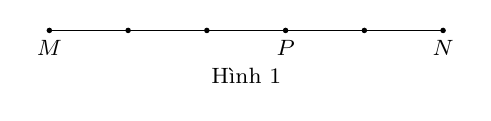
\begin{tikzpicture}[scale=1, font=\footnotesize, line join=round, line cap=round, >=stealth,x=1cm,y=1cm]
		\draw (0,0)node[below]{$M$}--(5,0)node[below]{$N$} (3,0)node[below]{$P$} (2.5,-.35)node[below]{Hình 1};
		\foreach \x in {0,1,2,3,4,5} {\fill (\x,0)circle(1pt);}
	\end{tikzpicture}
	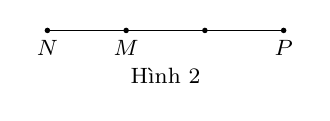
\begin{tikzpicture}[scale=1, font=\footnotesize, line join=round, line cap=round, >=stealth,x=1cm,y=1cm]
		\draw (0,0)node[below]{$N$}--(3,0)node[below]{$P$} (1,0)node[below]{$M$} (1.5,-.35)node[below]{Hình 2};
		\foreach \x in {0,1,2,3} {\fill (\x,0)circle(1pt);}
	\end{tikzpicture}\\[.5cm]
	
	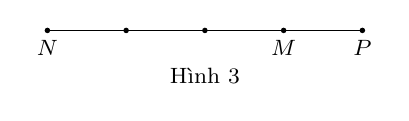
\begin{tikzpicture}[scale=1, font=\footnotesize, line join=round, line cap=round, >=stealth,x=1cm,y=1cm]
		\draw (0,0)node[below]{$N$}--(4,0)node[below]{$P$} (3,0)node[below]{$M$} (2,-.35)node[below]{Hình 3};
		\foreach \x in {0,1,2,3,4} {\fill (\x,0)circle(1pt);}
	\end{tikzpicture}
	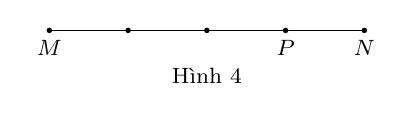
\begin{tikzpicture}[scale=1, font=\footnotesize, line join=round, line cap=round, >=stealth,x=1cm,y=1cm]
		\draw (0,0)node[below]{$M$}--(4,0)node[below]{$N$} (3,0)node[below]{$P$} (2,-.35)node[below]{Hình 4};
		\foreach \x in {0,1,2,3,4} {\fill (\x,0)circle(1pt);}
	\end{tikzpicture}
	\end{center}
	\choice
	{Hình $1$}
	{Hình $2$}
	{\True Hình $3$}
	{Hình $4$}
	\loigiai{
		Do $\vec{MN}=-3\vec{MP}$ nên $\vec{MN}$ ngược hướng với $\vec{MP}$ và $MN=3MP$.
	}
\end{ex}
%Câu 1...........................
\begin{ex}%[0T6Y1-1]%[Dự án đề kiểm tra HKII NH22-23- Nguyễn Sĩ Đạt]%[THPT Giồng Ông Tố]
		Khi sử dụng máy tính bỏ túi với $10$ chữ số thập phân ta được $\sqrt{8}=2{,}828427125$. Giá trị gần đúng của $\sqrt{8}$ chính xác đến hàng phần trăm là
		\choice
		{$2{,}84$}
		{$2{,}81$}
		{$2{,}82$}
		{\True $2{,}83$}
		\loigiai{
			Ta có $\sqrt{8}=2{,}828427125$ do đó giá trị gần đúng của $\sqrt{8}$ chính xác đến hàng phần trăm là $2{,}83$.
		}
\end{ex}
%Câu 1...........................
\begin{ex}%[0T3Y1-1]%[Dự án đề kiểm tra HKII NH22-23- Nguyễn Sĩ Đạt]%[THPT Giồng Ông Tố]
		Điểm nào sau đấy thuộc đồ thị hàm số $y=\dfrac{1}{x-1}$.
		\choice
		{$M_3(2;0)$}
		{$M_4(0;-2)$}
		{\True $M_1(2;1)$}
		{$M_2(1;1)$}
		\loigiai{
			Với $x=2$ thì $y=\dfrac{1}{2-1}=1$. Vậy $M_1(2;1)$ thuộc đồ thị hàm số đã cho.
		}
\end{ex}
%Câu 1...........................
\begin{ex}%[0T1B2-1]%[Dự án đề kiểm tra HKII NH22-23- Nguyễn Sĩ Đạt]%[THPT Giồng Ông Tố]
	Liệt kê các phần tử của tập hợp $X=\left\lbrace x\in\mathbb{N}\, | \,x-5\le-4x\right\rbrace $.
	\choice
	{$\varnothing$}
	{$\left\lbrace 0;1;2\right\rbrace $}
	{\True $\left\lbrace 0;1\right\rbrace $}
	{$\left\lbrace -1;0;1\right\rbrace $}
	\loigiai{
		Ta có
		$X=\left\lbrace x\in\mathbb{N}\, | \,x-5\le-4x\right\rbrace =\left\lbrace x\in\mathbb{N}\, | \,5x\le 5\right\rbrace =\left\lbrace x\in\mathbb{N}\, | \,x\le 1\right\rbrace =\left\lbrace 0;1\right\rbrace $.
	}
\end{ex}
%Câu 1...........................
\begin{ex}%[0T3B2-1]%[Dự án đề kiểm tra HKII NH22-23- Nguyễn Sĩ Đạt]%[THPT Giồng Ông Tố] 
		Bảng biến thiên của hàm số $y=-2x^2+4x+1$ là bảng nào sau đây
		\choice
		{
\begin{tikzpicture}
				\tkzTabInit[lgt=1.5,espcl=3,deltacl=1]{$x$/1 ,$y$/2}
				{$-\infty$ , $2$ , $+\infty$}
				\tkzTabVar{+/$+\infty$ , -/$1$ , +/$+\infty$}
		\end{tikzpicture}}
	{
\begin{tikzpicture}
			\tkzTabInit[lgt=1.5,espcl=3,deltacl=1]{$x$/1 ,$y$/2}
			{$-\infty$ , $1$ , $+\infty$}
			\tkzTabVar{+/$+\infty$ , -/$3$ , +/$+\infty$}
	\end{tikzpicture}}
	{\True 
\begin{tikzpicture}
			\tkzTabInit[lgt=1.5,espcl=3,deltacl=1]{$x$/1 ,$y$/2}
			{$-\infty$ , $1$ , $+\infty$}
			\tkzTabVar{-/$-\infty$ , +/$3$ , -/$-\infty$}
	\end{tikzpicture}}
	{
\begin{tikzpicture}
			\tkzTabInit[lgt=1.5,espcl=3,deltacl=1]{$x$/1 ,$y$/2}
			{$-\infty$ , $2$ , $+\infty$}
			\tkzTabVar{-/$-\infty$ , +/$1$ , -/$-\infty$}
	\end{tikzpicture}}
		\loigiai{
			Ta có $y=-2x^2+4x+1$ có hệ số $a=-2$, có tọa độ đỉnh là $I\left( 1;3\right) $.\\
			Vậy hàm số đồng biến trên khoảng $\left(-\infty;1\right)$ và nghịch biến trên khoảng $\left(1;+\infty\right)$.\\
			Giá trị lớn nhất của hàm số trên $\mathbb{R}$ là $f(1)=3$.
		} 
\end{ex}
%Câu 1...........................
\begin{ex}%[0T5Y4-1]%[Dự án đề kiểm tra HKII NH22-23- Nguyễn Sĩ Đạt]%[THPT Giồng Ông Tố] 
		Cho hai vectơ $\vec{a}$ và $\vec{b}$ thỏa mãn $\left| \vec{a}\right| =3$, $\left| \vec{b}\right| =2$ và $\vec{a} \cdot \vec{b}=-3$. Xác định góc $\alpha$ giữa hai vectơ $\vec{a}$ và $\vec{b}$.
		\choice
		{$\alpha=60^{\circ}$}
		{$\alpha=30^{\circ}$}
		{\True $\alpha=120^{\circ}$}
		{$ \alpha = 45^{\circ} $}
		\loigiai{
			Ta có 
			$
			\cos (\vec{a} ; \vec{b})=\dfrac{\vec{a} \cdot \vec{b}}{\left| \vec{a}\right|  \cdot\left| \vec{b}\right| } = \dfrac{-3}{3 \cdot 2}=-\dfrac{1}{2} \Rightarrow (\vec {a} ; \vec{b}) = 120^\circ .
			$
		} 
\end{ex}
%Câu 1...........................
\begin{ex}%[0T5B4-3]%[Dự án đề kiểm tra HKII NH22-23- Nguyễn Sĩ Đạt]%[THPT Giồng Ông Tố]
	Cho tam giác $ABC$ vuông tại $A$ và có $AB=c$, $AC=b$. Tính $\vec{BA}\cdot \vec{BC}$.
	\choice{$b^2-c^2$}{$b^2$}{$b^2+c^2$}{\True $c^2$}
	\loigiai{
		Vì tam giác $ABC$ vuông tại $A$ nên $AB \perp AC$. Suy ra $\vec{BA}\cdot \vec{AC}=0$.\\
		Ta có $\vec{BA}\cdot \vec{BC} = \vec{BA}\cdot\left(\vec{BA}+\vec{AC}\right) = \left(\vec{BA}\right)^2 + \vec{BA}\cdot \vec{AC} = BA^2 + 0 = c^2 $.
	}
\end{ex} 



%Câu 9...........................
\begin{ex}%[0T3Y2-3]%[Dự án đề kiểm tra HKII NH22-23- Nguyễn Cường]%[THPT Giồng Ông Tố]
Điểm $I(-2;1)$ là đỉnh của Parabol nào sau đây?
	\choice
	{$y=-x^2-4x+3$}
	{$y=x^2+4x-5$}
	{\True $y=x^2+4x+5$}
	{$y=2x^2+4x+1$}
	\loigiai{
		Parabol $y=x^2+4x+5$ có tọa độ đỉnh là $I(-2;1)$.
	}
\end{ex}
%Câu 20...........................
\begin{ex}%[0T6Y1-2]%[Dự án đề kiểm tra HKII NH22-23- Nguyễn Cường]%[THPT Giồng Ông Tố]
	Cho $a=46{,}7543$ và có độ chính xác $d=0{,}01$. Số quy tròn của $a$ là
	\choice
	{$46{,}75$}
	{$46{,}7$}
	{\True $46{,}8$}
	{$46{,}76$}
	\loigiai{
		Các bước xác định số quy tròn của số gần đúng $a$ với độ chính xác $d$ cho trước\\
		Buớc 1 : Tìm hàng của chữ số khác 0 đầu tiên bên trái của $d$.\\
		Buớc 2: Quy tròn số $a$ ở hàng gấp 10 lần hàng tìm được ở Bước 1 .\\
		Do đó, số quy tròn của $a$ với có độ chính xác $d=0{,}01$ là $46{,}8$.
	}
\end{ex}
%Câu 21...........................
\begin{ex}%[0T5B4-1]%[Dự án đề kiểm tra HKII NH22-23- Nguyễn Cường]%[THPT Giồng Ông Tố]
	Cho tam giác $ABC$ vuông tại $A$ và có $BC=2AC$. Tính $\cos\left(\overrightarrow{AC},\overrightarrow{CB}\right)$.
	\choice
	{\True $\cos\left(\overrightarrow{AC},\overrightarrow{CB}\right)=-\dfrac{1}{2}$}
	{$\cos\left(\overrightarrow{AC},\overrightarrow{CB}\right)=\dfrac{1}{2}$}
	{$\cos\left(\overrightarrow{AC},\overrightarrow{CB}\right)=\dfrac{\sqrt{3}}{2}$}
	{$\cos\left(\overrightarrow{AC},\overrightarrow{CB}\right)=-\dfrac{\sqrt{3}}{2}$}
	\loigiai{
	\immini
	{
	Ta có $\cos\left(\overrightarrow{AC},\overrightarrow{CB}\right)=-\cos\left(\overrightarrow{CA},\overrightarrow{CB}\right)=-\cos\widehat{ACB}=-\dfrac{AC}{BC}=-\dfrac{1}{2}$.
}
{
\begin{tikzpicture}[join = round, cap = round, >=stealth, font = \footnotesize, scale = .7]
	\path 
	(0,0) coordinate (A)
	+(0:3) coordinate (B)
	+(90:5) coordinate (C)
	;
	\draw (A)--(B)--(C)--cycle
	pic[draw,angle radius = 8pt]{right angle = B--A--C}
	;
	\foreach \x/\g in {A/180,B/0,C/90}
	\fill (\x) circle (1.5pt)
	+(\g:3mm) node{$\x$};
\end{tikzpicture}
}
	}
\end{ex}
%Câu 22...........................
\begin{ex}%[0T5Y1-3]%[Dự án đề kiểm tra HKII NH22-23- Nguyễn Cường]%[THPT Giồng Ông Tố]
	Gọi $O$ là giao điểm của hai đường chéo $AC$ và $BD$ của hình bình hành $ABCD$. Đẳng thức nào sau đây là \textbf{sai}?
	\choice
	{$\overrightarrow{AB}=\overrightarrow{DC}$}
	{\True $\overrightarrow{OA}=\overrightarrow{OC}$}
	{$\overrightarrow{OB}=\overrightarrow{DO}$}
	{$\overrightarrow{CB}=\overrightarrow{DA}$}
	\loigiai{
		\immini
		{
			Ta có $\overrightarrow{OA}$ và $\overrightarrow{OC}$ là hai véc-tơ đối nhau, do đó $\overrightarrow{OA}=\overrightarrow{OC}$ là khẳng định sai.
		}
		{
			\begin{tikzpicture}[join = round, cap = round, >=stealth, font = \footnotesize, scale = .7]
	\path 
	(0:0) coordinate (D)
	+(0:5) coordinate (C)
	+(65:3) coordinate (A)
	($(A)+(C)-(D)$) coordinate (B)
	($(A)!.5!(C)$)coordinate (O) 
	;
	\draw 
	(A)--(B)--(C)--(D)--cycle
	(A)--(C) (B)--(D)
	;
	\foreach \x/\g in {D/-90,C/-90,A/90,B/90,O/-90}
	\fill (\x) circle (1.5pt)
	+(\g:3mm) node{$\x$};
\end{tikzpicture}\
		}
	}
\end{ex}
%Câu 23...........................
\begin{ex}%[0T4B3-1]%[Dự án đề kiểm tra HKII NH22-23- Nguyễn Cường]%[THPT Giồng Ông Tố]
Tam giác $ABC$ vuông cân tại $A$, có $AB=a$. Tính bán kính $r$ của đường tròn nội tiếp tam giác $ABC$.
	\choice
	{$r=\dfrac{a}{\sqrt{2}}$}
	{\True $r=\dfrac{a}{2+\sqrt{2}}$}
	{$r=\dfrac{a}{2}$}
	{$r=\dfrac{a}{3}$}
	\loigiai{
		\immini
		{
		Ta có $BC=\sqrt{AB^2+AC^2}=a\sqrt{2}$.\\
		Diện tích tam giác $ABC$ là $S=\dfrac{1}{2}AB\cdot AC=\dfrac{a^2}{2}$.\\
		Nửa chu vi tam giác $ABC$ là $$p=\dfrac{AB+BC+CA}{2}=\dfrac{a+a\sqrt{2}+a}{2}=\dfrac{a\left(2+\sqrt{2}\right)}{2}.$$
		Mà ta lại có $S=pr\Leftrightarrow r=\dfrac{S}{p}=\dfrac{a}{2+\sqrt{2}}$.
		}
			{
				\begin{tikzpicture}[join = round, cap = round, >=stealth, font = \footnotesize, scale = .7]
					\path 
					(0,0) coordinate (A)
					+(0:3) coordinate (B)
					+(90:3) coordinate (C)
					;
					\draw (A)--(B)--(C)--cycle
					pic[draw,angle radius = 8pt]{right angle = B--A--C}
					;
					\foreach \x/\g in {A/180,B/0,C/90}
					\fill (\x) circle (1.5pt)
					+(\g:3mm) node{$\x$};
				\end{tikzpicture}
			}
		}
	\end{ex}
%Câu 24...........................
\begin{ex}%[0T3B2-2]%[Dự án đề kiểm tra HKII NH22-23- Nguyễn Cường]%[THPT Giồng Ông Tố]
	Cho parabol $(P)\colon y=ax^2+bx+2$ với $a\ne 0$. Biết rằng parabol đó đi qua hai điểm $A(1;5)$ và $B(-2;8)$. Parabol đó là
	\choice
	{\True $y=2x^2+x+2$}
	{$y=x^2-4x+2$}
	{$y=-x^2+2x+2$}
	{$y=x^2-3x+2$}
	\loigiai{
	Ta có $\heva{&a+b+2=5\\&4a-2b+2=8}\Leftrightarrow\heva{&a+b=3\\&4a-2b=6}\Leftrightarrow\heva{&a=2\\&b=1.}$\\
	Vậy parabol là $y=2x^2+x+2$.
		}
	\end{ex}
%Câu 25...........................
\begin{ex}%[0T5B2-2]%[Dự án đề kiểm tra HKII NH22-23- Nguyễn Cường]%[THPT Giồng Ông Tố]
	Cho bốn điểm $A$, $B$, $C$, $D$ phân biệt. Khi đó $\overrightarrow{AB}-\overrightarrow{DC}+\overrightarrow{BC}-\overrightarrow{AD}$ bàng véc-tơ nào sau đây?
	\choice
	{$2\overrightarrow{DC}$}
	{\True $\overrightarrow{0}$}
	{$\overrightarrow{AC}$}
	{$\overrightarrow{BD}$}
	\loigiai{
		Ta có \allowdisplaybreaks
		\begin{eqnarray*}
			&&\overrightarrow{AB}-\overrightarrow{DC}+\overrightarrow{BC}-\overrightarrow{AD}\\
			&=&\overrightarrow{AB}+\overrightarrow{CD}+\overrightarrow{BC}+\overrightarrow{DA}\\
			&=&\overrightarrow{AB}+\overrightarrow{BC}+\overrightarrow{CD}+\overrightarrow{DA}\\
			&=&\overrightarrow{0}.
		\end{eqnarray*}
	}
\end{ex}
%Câu 26...........................
\begin{ex}%[0T3B1-1]%[Dự án đề kiểm tra HKII NH22-23- Nguyễn Cường]%[THPT Giồng Ông Tố]
	Cho hàm số $f(x)=2x^2+3x+1$ và $g(x)=\heva{&x^2+1&&\text{khi }x>2\\&2x-1&&\text{khi }-2\le x\le 2\\&6-5x&&\text{khi }x<-2}$. Tính các giá trị $f(-1)$ và $g(-3)$, $g(2)$, $g(3)$ 
	\choice
	{\True $f(-1)=0$, $g(-3)=21$, $g(2)=3$, $g(3)=10$}
	{$f(-1)=1$, $g(-3)=32$, $g(2)=5$, $g(3)=17$}
	{$f(-1)=-1$, $g(-3)=34$, $g(2)=3$, $g(3)=8$}
	{$f(-1)=-1$, $g(-3)=12$, $g(2)=41$, $g(3)=7$}
	\loigiai{
		\begin{itemize}
			\item $f(-1)=2\cdot (-1)^2+3\cdot (-1)+1=0$.
			\item $g(-3)=6-5\cdot(-3)=21$.
			\item $g(2)=2\cdot 2-1=3$.
			\item $g(3)=3^2+1=10$.
		\end{itemize}
	}
\end{ex}
%Câu 27...........................
\begin{ex}%[0T5B3-4]%[Dự án đề kiểm tra HKII NH22-23- Nguyễn Cường]%[THPT Giồng Ông Tố]
	Cho tam giác $ABC$. Gọi $M$ là điểm trên cạnh $BC$ sao cho $MB=3MC$. Khi đó, biểu diễn $\overrightarrow{AM}$ theo $\overrightarrow{AB}$ và $\overrightarrow{AC}$ ta được
	\choice
	{$\overrightarrow{AM}=\dfrac{1}{4}\overrightarrow{AB}+\dfrac{1}{6}\overrightarrow{AC}$}
	{\True $\overrightarrow{AM}=\dfrac{1}{4}\overrightarrow{AB}+\dfrac{3}{4}\overrightarrow{AC}$}
	{$\overrightarrow{AM}=\dfrac{1}{4}\overrightarrow{AB}+3\overrightarrow{AC}$}
	{$\overrightarrow{AM}=\dfrac{1}{2}\overrightarrow{AB}+\dfrac{1}{6}\overrightarrow{AC}$}
	\loigiai{
		\immini
		{
	Gọi $N$ là trung điểm $BC$, khi đó $M$ là trung điểm của $NC$. Ta có
	\allowdisplaybreaks
	\begin{eqnarray*}
		\overrightarrow{AM}&=&\dfrac{1}{2}\overrightarrow{AN}+\dfrac{1}{2}\overrightarrow{AC}\\
		&=&\dfrac{1}{2}\left(\dfrac{1}{2}\overrightarrow{AB}+\dfrac{1}{2}\overrightarrow{AC}\right)+\dfrac{1}{2}\overrightarrow{AC}\\
		&=&\dfrac{1}{4}\overrightarrow{AB}+\dfrac{3}{4}\overrightarrow{AC}.
	\end{eqnarray*}
	}
{
\begin{tikzpicture}[join = round, cap = round, thick, font = \small, scale = 1]
	\path (0:0) coordinate (B)
	+(0:5) coordinate (C)
	+(70:3) coordinate (A)
	($(B)!3/4!(C)$)coordinate(M)
	($(B)!1/2!(C)$)coordinate(N)
	;
	\draw (A)--(B)--(C)--cycle
	;
	\draw [->](A)--(M);
	\foreach \x/\g in {B/180,C/0,A/90,M/90,N/90}
	\fill (\x) circle (1.5pt)
	+(\g:3mm) node{$\x$};
\end{tikzpicture}

}
	}
\end{ex}


\begin{ex}%[Dự án đề kiểm tra HKII-NH22-23, Dương Phước Sang]%[THPT Giồng Ông Tố-TP.HCM]%[0T3B2-3]
		Cho hàm số $y=ax^2+bx+c$ $(a > 0)$. Khẳng định nào sau đây là \textbf{sai}?
		\choice
		{Hàm số đồng biến trên khoảng $\left(-\dfrac{b}{2a};+\infty\right)$}
		{Đồ thị hàm số có trục đối xứng là đường thẳng $x=-\dfrac{b}{2a}$}
		{\True Đồ thị hàm số luôn cắt trục hoành tại $2$ điểm phân biệt}
		{Hàm số nghịch biến trên khoảng $\left(-\infty;-\dfrac{b}{2a}\right)$}
		\loigiai{
			Khẳng định ``đồ thị hàm số $y=ax^2+bx+c$ $(a > 0)$ luôn cắt trục hoành tại $2$ điểm phân biệt'' là sai.\\
			Chẳng hạn, xét hàm số $y=x^2+2x+9$ có hệ số $a=1>0$ nhưng $x^2+2x+9=(x+1)^2+8>0$ với mọi $x \in \mathbb{R}$, do đó đồ thị hàm số không có điểm chung với trục hoành.
		}
	\end{ex}

	\begin{ex}%[Dự án đề kiểm tra HKII-NH22-23, Dương Phước Sang]%[THPT Giồng Ông Tố-TP.HCM]%[0T3Y1-2]
		Tập xác định của hàm số $y=\dfrac{x+1}{x-1}$ là
		\choice
		{\True $\mathbb{R} \setminus \big\{1\big\}$}
		{$(1;+\infty)$}
		{$\mathbb{R} \setminus \big\{-1\big\}$}
		{$\mathbb{R} \setminus \big\{-1;1\big\}$}
		\loigiai{
			Hàm số $y=\dfrac{x+1}{x-1}$ có nghĩa khi và chỉ khi $x-1 \neq 0 \Leftrightarrow x \neq 1$.\\
			Tập xác định của hàm số $y=\dfrac{x+1}{x-1}$ là $\mathscr{D}=\mathbb{R} \setminus \big\{1\big\}$.
		}
	\end{ex}

	\begin{ex}%[Dự án đề kiểm tra HKII-NH22-23, Dương Phước Sang]%[THPT Giồng Ông Tố-TP.HCM]%[0T5B2-5]
		Cho hình vuông $ABCD$ cạnh $a$, tâm $O$. Khi đó $\left|\overrightarrow{OA}-\overrightarrow{BO}\right|$ bằng
		\choice
		{$a\sqrt{2}$}
		{$2a$}
		{$\dfrac{a}{2}$}
		{\True $a$}
		\loigiai{
			\immini{
				Do $ABCD$ là hình vuông tâm $O$ nên $\overrightarrow{OB}=\overrightarrow{DO}$.\\
				Ta có $\left|\overrightarrow{OA}-\overrightarrow{BO}\right|=\left|\overrightarrow{OA}+\overrightarrow{OB}\right|=\left|\overrightarrow{OA}+\overrightarrow{DO}\right|=\left|\overrightarrow{DA}\right|=a$.}
			{\vspace{-0.5cm}
				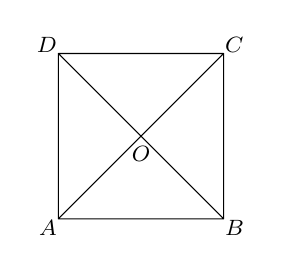
\begin{tikzpicture}[scale=0.7, font=\footnotesize, line join=round, line cap=round]
					\draw (0,0)node[below left=-3pt]{$A$}--(3,0)node[below right=-3pt]{$B$}--(3,3)node[above right=-3pt]{$C$}--(0,3)node[above left=-3pt]{$D$}--(0,0)--(3,3) (0,3)--(3,0);
					\node at (1.5,1.5)[below]{$O$};
			\end{tikzpicture}}
		}
	\end{ex}

	\begin{ex}%[Dự án đề kiểm tra HKII-NH22-23, Dương Phước Sang]%[THPT Giồng Ông Tố-TP.HCM]%[0T1Y2-3]
		Cho tập hợp $A=[9;+\infty)$. Hãy viết lại tập hợp $A$ dưới dạng nêu tính chất đặc trưng.
		\choice
		{$A=\big\{x \in \mathbb{R} \mid 9 \leq x \leq +\infty\big\}$}
		{$A=\big\{x \in \mathbb{R} \mid x \leq 9\big\}$}
		{\True $A=\big\{x \in \mathbb{R} \mid x \geq 9\big\}$}
		{$A=\big\{x \in \mathbb{R} \mid x<9\big\}$}
		\loigiai{
			Ta có $A=[9;+\infty)=\big\{x \in \mathbb{R} \mid x \geq 9\big\}$.
		}
	\end{ex}

	\begin{ex}%[Dự án đề kiểm tra HKII-NH22-23, Dương Phước Sang]%[THPT Giồng Ông Tố-TP.HCM]%[0T2Y1-1]
		Hệ nào sau đây \textbf{không phải} là hệ bất phương trình bậc nhất hai ẩn?
		\choice
		{\True $\heva{&5x+y-9=0\\&4x-7y+3=0}$}
		{$\heva{&3x+y-1 \leq 0\\&2x-y+2 \geq 0}$}
		{$\heva{&y-1<0\\&x+2 \geq 0}$}
		{$\heva{&x+y-3 \leq 0\\&-2x+y+3 \geq 0\\&x \geq 0,\;y \geq 0}$}
		\loigiai{
			Hệ $\heva{&5x+y-9=0\\&4x-7y+3=0}$ là hệ phương trình bậc nhất theo $2$ ẩn $x,y$, không phải hệ bất phương trình bậc nhất hai ẩn.
		}
	\end{ex}

	\begin{ex}%[Dự án đề kiểm tra HKII-NH22-23, Dương Phước Sang]%[THPT Giồng Ông Tố-TP.HCM]%[0T4Y2-2]
		Cho tam giác $ABC$ có $BC=a$, $AC=b$ và $AB=c$; $R$ là bán kính đường tròn ngoại tiếp tam giác $ABC$. Tìm công thức \textbf{sai}.
		\choice
		{$\dfrac{a}{\sin A}=2R$}
		{$\sin A=\dfrac{a}{2R}$}
		{$\sin C=\dfrac{c\,\sin A}{a}$}
		{\True $b\,\sin B=2R$}
		\loigiai{
			Theo định lý sin ta có $\dfrac{a}{\sin A}=\dfrac{b}{\sin B}=\dfrac{c}{\sin C}=2R$, do đó $b\,\sin B=2R$ là công thức sai.
		}
	\end{ex}

	\begin{ex}%[Dự án đề kiểm tra HKII-NH22-23, Dương Phước Sang]%[THPT Giồng Ông Tố-TP.HCM]%[0T4Y2-2]
		Cho tam giác $ABC$ có $BC=a$, $AC=b$ và $AB=c$; $S$ là diện tích tam giác $ABC$. Chọn công thức \textbf{sai}.
		\choice
		{$\cos C=\dfrac{a^2+b^2-c^2}{2ab}$}
		{$S=\dfrac{1}{2}bc\,\sin A$}
		{\True $S=\dfrac{1}{2}ab\,\cos C$}
		{$\cos A=\dfrac{b^2+c^2-a^2}{2bc}$}
		\loigiai{
			$S=\dfrac{1}{2}ab\,\sin C$ mới là công thức tính diện tích tam giác $ABC$, $S=\dfrac{1}{2}ab\,\cos C$ là công thức sai.
		}
	\end{ex}

	\begin{ex}%[Dự án đề kiểm tra HKII-NH22-23, Dương Phước Sang]%[THPT Giồng Ông Tố-TP.HCM]%[0T3B1-4]
		Trong các hàm số sau đây, hàm số nào đồng biến trên $\mathbb{R}$?
		\choice
		{$y=-2(2x-3)$}
		{$y=1-2x$}
		{$y=x^2+2x-1$}
		{\True $y=3x+2$}
		\loigiai{
			$y=3x+2$ là hàm số bậc nhất có hệ số góc $a=3>0$ nên đồng biến trên $\mathbb{R}$.
		}
	\end{ex}



\Closesolutionfile{ans}
%\begin{center}
%	\textbf{ĐÁP ÁN}
%	\inputansbox{10}{ans/ans}	
%\end{center}



\begin{center}
	\textbf{PHẦN 2 - TỰ LUẬN}
\end{center}


% Câu 1 - Tự luận
\begin{bt}%[0T3B1-2]%[Dự án đề kiểm tra HKI NH22-23 - Quan Ón]%[Giồng Ông Tố]
	Tìm tập xác định của hàm số $y = \dfrac{x - 1}{x^2 - 2x - 3}$.
	\dapso{$\mathscr{D} = \mathbb{R}\setminus \left\lbrace -1;3 \right\rbrace$.}
	\loigiai{
		Điều kiện xác định của hàm số là $x^2 - 2x - 3 \neq 0 \Leftrightarrow \heva{&x \neq -1\\&x \neq 3.}$\\
		Vậy tập xác định của hàm số đã cho là $\mathscr{D} = \mathbb{R}\setminus \left\lbrace -1;3 \right\rbrace$.
	}
\end{bt}

% Câu 2 - Tự luận
\begin{bt}%[0T3B2-5]%[Dự án đề kiểm tra HKI NH22-23 - Quan Ón]%[Giồng Ông Tố]
	Một quả bóng được cầu thủ sút lên rồi rơi xuống theo quỹ đạo là một parabol. Biết rằng ban đầu quả bóng được sút lên từ độ cao $1$ m, sau đó $1$ giây nó đạt độ cao $10$ m và sau $3{,}5$ giây nó ở độ cao $6{,}25$ m. Hỏi độ cao cao nhất mà quả bóng đạt được là bao nhiêu mét?
	\dapso{$13$ m.}
	\loigiai{
	    \immini{
	    Theo giả thiết, quỹ đạo của quả bóng là một parabol nên có phương trình dạng $y = ax^2 + bx + c$ ($a\neq 0$).\\
	    Gọi $A(0;1)$, $B\left( 1;10 \right)$, $C\left(3{,}5; 6{,}25 \right)$ lần lượt là các vị trí của quả bóng tại thời điểm $0$ giây, $1$ giây và $3{,}5$ giây.\\
	    Vì parabol đi qua ba điểm $A$, $B$, $C$ nên ta có hệ phương trình
	    $$ \heva{&1 = a\cdot 0^2 + b\cdot 0 + c\\&10 = a\cdot 1^2 + b\cdot 1 + c\\&6{,}25 = a\cdot 3{,}5^2 + b\cdot 3{,}5 + c} \Leftrightarrow \heva{&c = 1\\&a + b + c = 10\\&\dfrac{49}{4}a + \dfrac{7}{2}b + c = \dfrac{25}{4}} \Leftrightarrow \heva{&a = -3\\&b = 12\\&c = 1.} $$
	    Suy ra phương trình của parabol là $y = -3x^2 + 12x + 1$.\\
	    Parabol có đỉnh $I(2;13)$ nên quả bóng đạt độ cao cao nhất tại $h = 13$ m.
    }{
        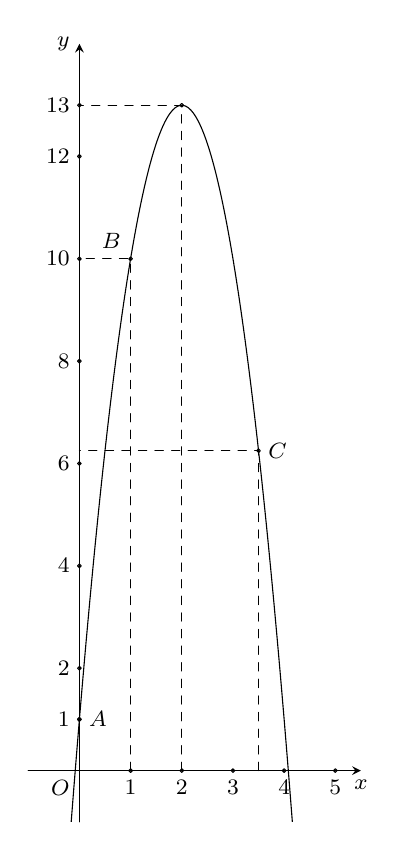
\begin{tikzpicture}[scale=0.65, font=\footnotesize, line join=round, line cap=round, >=stealth]
        	\def\xt{-1} \def\xp{5.5} \def\yt{14.2} \def\yd{-1}
        	\draw[->] (\xt,0)--(\xp,0) node [below]{$x$};
        	\draw[->] (0,\yd)--(0,\yt) node [left]{$y$};
        	\node at (0,0) [below left]{$O$} circle (1pt);
        	\foreach \x in {1,2,3,4,5}{
        		\draw (\x,0) node[below]{$\x$} circle (1pt);
        	}
        	\foreach \x in {1,2,4,6,8,10,12,13}{
        		\draw (0,\x) node[left]{$\x$} circle (1pt);
        	}
        	\draw (0,1) node[right]{$A$} circle (1pt);
        	\draw (1,10) node[above left]{$B$} circle (1pt);
        	\draw (3.5,6.25) node[right]{$C$} circle (1pt);
        	\draw (2,13) circle (1pt);
        	\clip (\xt,\yd) rectangle (\xp,\yt);
        	\draw[dashed] (1,0)--(1,10)--(0,10) (2,0)--(2,13)--(0,13) (3.5,0)--(3.5,6.25)--(0,6.25);
        	\draw [smooth, domain=-0.5:4.5, samples=100] %
        	plot (\x, {-3*(\x)^2 + 12*(\x) + 1});
        \end{tikzpicture}
}
	}
\end{bt}

% Câu 3 - Tự luận
\begin{bt}%[0T5B3-4]%[Dự án đề kiểm tra HKI NH22-23 - Quan Ón]%[Giồng Ông Tố]
	Cho hình bình hành $ABCD$ có $E$, $N$ lần lượt là trung điểm của $BC$, $AE$. Tìm các số $p$ và $q$ sao cho $\overrightarrow{DN} = p\overrightarrow{AB} + q\overrightarrow{AC}$.
	\dapso{$p = \dfrac{5}{4}$; $q = -\dfrac{3}{4}$.}
	\loigiai{
	    \immini{
	    Ta có
	    \begin{eqnarray*}
	    	\overrightarrow{DN} &=& \overrightarrow{DA} + \overrightarrow{AN}\\
	    	&=& \overrightarrow{CB} + \dfrac{1}{2}\overrightarrow{AE}\\
	    	&=& \overrightarrow{AB} - \overrightarrow{AC} + \dfrac{1}{2}\cdot \dfrac{1}{2}\left( \overrightarrow{AB} + \overrightarrow{AC} \right)\\
	    	&=& \overrightarrow{AB} - \overrightarrow{AC} + \dfrac{1}{4}\left( \overrightarrow{AB} + \overrightarrow{AC} \right)\\
	    	&=& \overrightarrow{AB} - \overrightarrow{AC} + \dfrac{1}{4}\overrightarrow{AB} + \dfrac{1}{4}\overrightarrow{AC} \\
	    	&=& \dfrac{5}{4}\overrightarrow{AB} - \dfrac{3}{4}\overrightarrow{AC}.
	    \end{eqnarray*}
	    Vậy $p = \dfrac{5}{4}$; $q = -\dfrac{3}{4}$.
    }{
        \begin{tikzpicture}[>=stealth,line join=round,line cap=round,font=\footnotesize,scale=1]
        	\path
        	(0,2.5) coordinate (A)
        	(4,2.5) coordinate (B)
        	(3,0) coordinate (C)
        	(-1,0) coordinate (D)
        	($(B)!0.5!(C)$) coordinate (E)
        	($(A)!0.5!(E)$) coordinate (N);
        	\draw (A)--(B)--(C)--(D)--(A)--(C) (A)--(E);
        	\foreach \p/\r in {A/135,B/45,C/-45,D/-135,N/90,E/0}
        	\fill (\p) circle (1.2pt) node[shift={(\r:3mm)}]{$\p$};
        \end{tikzpicture}
}
	}
\end{bt}

% Câu 4 - Tự luận
\begin{bt}%[0T5T4-1]%[Dự án đề kiểm tra HKI NH22-23 - Quan Ón]%[Giồng Ông Tố]
	Tính công sinh bởi một lực $\overrightarrow{F}$ có độ lớn $60$ N kéo một vật dịch chuyển một véc-tơ $\overrightarrow{d}$ có độ dài $200$ m. Cho biết $\left( \overrightarrow{F}, \overrightarrow{d} \right) = 60^\circ$.
	\dapso{$6000$ J.}
	\loigiai{
		Công sinh bởi lực $\overrightarrow{F}$ là
		$$ \overrightarrow{F}\cdot \overrightarrow{d} = \left|\overrightarrow{F} \right|\cdot \left|\overrightarrow{d} \right|\cdot \cos 60^\circ = 60\cdot 200\cdot \dfrac{1}{2} = 6000 \quad \textrm{(J).}$$
	}
\end{bt}


